\scanpage{119}
% archive foliation: 118
\uline{degré $6$}\quad a) $1$ sommet d’ordre $6$
\figure{\begin{tikzpicture}[scale=.64,line cap=round,line join=round]\begin{scope}[shift={(6,3)}]\fill(0,0)circle(2pt);\draw(0,0)--(30:.8);\draw(0,0)--(90:.8);\draw(0,0)--(150:.8);\draw(0,0)--(210:.8);\draw(0,0)--(270:.8);\draw(0,0)--(330:.8);\node at(0,-1){$\uuline{D_6}$};\end{scope}\begin{scope}[shift={(9,3)}]\fill(0,0)circle(2pt);\draw(0,0)..controls(1.3,1.4)and(1.4,-1)..(0,0);\draw(-.7,.4)--(0,0)--(-.7,-.4);\draw(0,-.7)--(0,0)--(.4,-.6);\node at(0,-1){$\mathbb Z_2$};\end{scope}\begin{scope}[shift={(12,3)}]\fill(0,0)circle(2pt);\draw(0,0)..controls(1.3,1.4)and(1.4,-1)..(0,0);\draw(-.7,.2)--(0,0)--(.5,.1);\draw(-.5,-.6)--(0,0)--(0,-.7);\node at(0,-1){$\mathbb Z_2$};\end{scope}\begin{scope}[shift={(0,1.1)}]\fill(0,0)circle(2pt);\draw(0,0)..controls(1.3,1.4)and(1.4,-1)..(0,0);\draw(-.7,.3)--(0,0)--(.6,.2);\draw(-.7,-.4)--(0,0)--(.6,-.2);\node at(0,-1){$\mathbb Z_2\times\mathbb Z_2$};\end{scope}\begin{scope}[shift={(3.1,1.1)}]\fill(0,0)circle(2pt);\draw(0,0)..controls(-1.2,1.3)and(-1.5,-1.2)..(0,0)..controls(1.4,1.2)and(1.4,-1.2)..(0,0);\draw(-.6,-.6)--(0,0)--(0,-.8);\node at(0,-1){$\mathbb Z_2$};\end{scope}\begin{scope}[shift={(6.5,1.1)}]\fill(0,0)circle(2pt);\draw(0,0)..controls(-1.2,1.3)and(-1.5,-1.2)..(0,0)..controls(1.4,1.2)and(1.4,-1.2)..(0,0);\draw(.7,.2)--(0,0)--(.6,-.2);\node at(1.2,-.7){$\times$};\node at(0,-1){$\mathbb Z_2$};\end{scope}\begin{scope}[shift={(10,1.1)}]\fill(0,0)circle(2pt);\draw(0,0)..controls(-1.2,1.3)and(-1.5,-1.2)..(0,0)..controls(1.4,1.2)and(1.4,-1.2)..(0,0);\draw(-.7,0)--(.7,.2);\node at(0,-1){$\mathbb Z_2\times\mathbb Z_2$};\end{scope}\begin{scope}[shift={(0,-1.3)}]\fill(0,0)circle(2pt);\draw(0,0)..controls(-1.2,1.3)and(-1.5,-1.2)..(0,0)..controls(1.4,1.2)and(1.4,-1.2)..(0,0);\draw(0,.7)--(0,0)--(.7,0);\node at(-1.2,-.8){$\times$};\node[draw,circle]at(0,-1){$1$};\end{scope}\begin{scope}[shift={(3,-1.3)}]\fill(0,0)circle(2pt);\draw(0,0)..controls(-1.2,1.3)and(-1.5,-1.2)..(0,0)..controls(1.4,1.2)and(1.4,-1.2)..(0,0);\draw(0,0)..controls(-.5,-1.7)and(.6,-1.7)..(0,0);\node at(0,-1){$\mathfrak S_3$};\end{scope}\begin{scope}[shift={(6.5,-1.3)}]\fill(0,0)circle(2pt);\draw(0,0)..controls(-1.2,1.3)and(-1.5,-1.2)..(0,0)..controls(1.4,1.2)and(1.4,-1.2)..(0,0);\draw(0,0)..controls(1.1,.7)and(1.1,-.7)..(0,0);\node at(0,-1){$\mathbb Z_2$};\end{scope}\begin{scope}[shift={(10.6,-1.6)}]\fill(0,0)circle(2pt);\draw(0,0)..controls(-1.2,1.3)and(-1.5,-1.2)..(0,0)..controls(1.4,1.2)and(1.4,-1.2)..(0,0);\draw(0,-.8)--(0,.8);\node at(0,-1){$\mathbb Z_2\times\mathbb Z_2$};\end{scope}\draw(7.5,3.8)--(7,2.5);\draw(7.6,3.8)--(7.1,2.5);\draw(1.7,2)--(1.7,.3);\draw(1.8,2)--(1.8,.3);\draw(1.5,-.5)--(1.1,-2.3);\draw(1.6,-.5)--(1.2,-2.3);\draw(12.1,1.5)--(12.2,.1);\foreach\y in{.2,.4,...,1.5}\draw(12,\y)--(12.3,\y+.15);\draw(1.9,2.1)..controls(4,2.4)and(4,1.1)..(4.8,.4)..controls(7,-.2)and(9.8,-.3)..(11.5,-.3)..controls(12.7,-2.7)..(11.4,-2.7)--(9.3,-2.7)..controls(8.8,-2.7)and(9,-1.5)..(8.5,-1)..controls(7,.1)and(4,-.2)..(3,-.25)..controls(1.5,-.4)..(1.9,2.1);\node at(10.5,-3.4){$\left(6,\begin{smallmatrix}2_2\\1_2\end{smallmatrix},\begin{smallmatrix}\unsure4\\\unsure{1_2}\end{smallmatrix}\right)$};\end{tikzpicture}}
b) $1$ sommet d’ordre $5$, $1$ d’ordre $1$
\figure{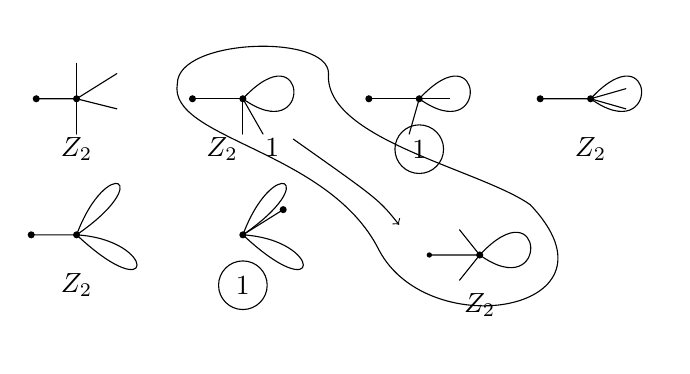
\begin{tikzpicture}[scale=.64,line cap=round,line join=round]\begin{scope}[shift={(0,1.5)}]\fill(0,0)circle(2pt);\draw(-.8,0)--(0,0)--(.8,.5);\draw(0,-.7)--(0,.7);\draw(0,0)--(.8,-.2);\fill(-.8,0)circle(2pt);\node at(0,-1){$\mathbb Z_2$};\end{scope}\begin{scope}[shift={(3.3,1.5)}]\fill(0,0)circle(2pt);\draw(0,0)..controls(1.3,1.4)and(1.4,-1)..(0,0);\draw(-1,0)--(0,0)--(0,-.7);\draw(0,0)--(.4,-.7);\fill(-1,0)circle(2pt);\node at(0,-1){$\deleted{\unsure{\mathbb Z_2}}\quad1$};\end{scope}\begin{scope}[shift={(6.8,1.5)}]\fill(0,0)circle(2pt);\draw(0,0)..controls(1.3,1.4)and(1.4,-1)..(0,0);\draw(-1,0)--(.6,0);\draw(0,0)--(-.2,-.7);\fill(-1,0)circle(2pt);\node[draw,circle]at(0,-1){$1$};\end{scope}\begin{scope}[shift={(10.2,1.5)}]\fill(0,0)circle(2pt);\draw(0,0)..controls(1.3,1.4)and(1.4,-1)..(0,0);\draw(-1,0)--(0,0)--(.7,.2);\draw(0,0)--(.7,-.2);\fill(-1,0)circle(2pt);\node at(0,-1){$\mathbb Z_2$};\end{scope}\begin{scope}[shift={(0,-1.2)}]\fill(0,0)circle(2pt);\draw(-.9,0)--(0,0)..controls(.6,1.6)and(1.6,1.1)..(0,0)..controls(1.6,-.1)and(1.6,-1.5)..(0,0);\fill(-.9,0)circle(2pt);\node at(0,-1){$\mathbb Z_2$};\end{scope}\begin{scope}[shift={(3.3,-1.2)}]\fill(0,0)circle(2pt);\draw(0,0)..controls(.6,1.6)and(1.6,1.1)..(0,0)..controls(1.6,-.1)and(1.6,-1.5)..(0,0);\draw(0,0)--(.8,.5);\fill(.8,.5)circle(2pt);\node[draw,circle]at(0,-1){$1$};\end{scope}\begin{scope}[shift={(8,-1.6)}]\fill(0,0)circle(2pt);\draw(0,0)..controls(1.3,1.4)and(1.4,-1)..(0,0);\draw(-1,0)--(0,0)--(-.4,.5);\draw(0,0)--(-.4,-.5);\fill(-1,0)circle(1.5pt);\node at(0,-1){$\mathbb Z_2$};\end{scope}\draw(2,1.8)..controls(2,2.7)and(5,2.8)..(5,2)..controls(4.9,.7)and(8,.1)..(9,-.6)..controls(11,-2.7)and(7,-3.4)..(6,-1.5)..controls(5,.5)and(1.8,.7)..(2,1.8);\draw[->](4.3,.7)..controls(6,-.5)..(6.4,-1);\end{tikzpicture}}
c) $1$ sommet d’ordre $4$, $1$ d’ordre $2$
\figure{\begin{tikzpicture}[scale=.64,line cap=round,line join=round]\begin{scope}[shift={(0,0)}]\fill(0,0)circle(2pt);\draw(-1.5,0)--(.9,0);\draw(.8,.6)--(0,0)--(.8,-.6);\fill(-.8,0)circle(2pt);\node at(0,-1){$\mathbb Z_2$};\end{scope}\begin{scope}[shift={(4,0)}]\fill(0,0)circle(2pt);\draw(0,0)..controls(1.3,1.4)and(1.4,-1)..(0,0);\draw(-1.5,0)--(0,0)--(.6,-.7);\fill(-.8,0)circle(2pt);\node[draw,circle]at(0,-1){$1$};\end{scope}\begin{scope}[shift={(8,0)}]\fill(0,0)circle(2pt);\draw(0,0)..controls(1.3,1.4)and(1.4,-1)..(0,0);\draw(-1.5,0)--(.5,0);\fill(-.8,0)circle(2pt);\node at(0,-1){$\mathbb Z_2$};\end{scope}\end{tikzpicture}}
\margin{\figure{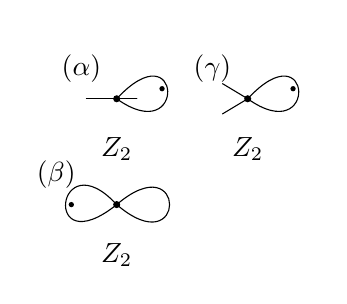
\begin{tikzpicture}[scale=.64,line cap=round,line join=round]\begin{scope}[shift={(-1,1.7)}]\fill(0,0)circle(2pt);\draw(0,0)..controls(1.3,1.4)and(1.4,-1)..(0,0);\draw(-.6,0)--(.4,0);\fill(.9,.2)circle(1.5pt);\node at(-.7,.6){$(\alpha)$};\node at(0,-1){$\mathbb Z_2$};\end{scope}\begin{scope}[shift={(1.6,1.7)}]\fill(0,0)circle(2pt);\draw(0,0)..controls(1.3,1.4)and(1.4,-1)..(0,0);\draw(-.5,.3)--(0,0)--(-.5,-.3);\fill(.9,.2)circle(1.5pt);\node at(-.7,.6){$(\gamma)$};\node at(0,-1){$\mathbb Z_2$};\end{scope}\begin{scope}[shift={(-1,-0.4)}]\fill(0,0)circle(2pt);\draw(0,0)..controls(-1.2,1.3)and(-1.5,-1.2)..(0,0)..controls(1.4,1.2)and(1.4,-1.2)..(0,0);\fill(-.9,0)circle(1.5pt);\node at(-1.2,.6){$(\beta)$};\node at(0,-1){$\mathbb Z_2$};\end{scope}\end{tikzpicture}}}
d) $1$ sommet d’ordre $4$, deux d’ordre $1$
\figure{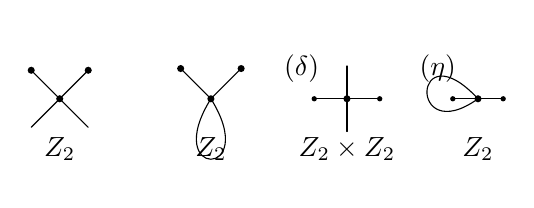
\begin{tikzpicture}[scale=.64,line cap=round,line join=round]\begin{scope}[shift={(0,0)}]\fill(0,0)circle(2pt);\foreach\a in{45,135,225,315}\draw(0,0)--(\a:.8);\fill(45:.8)circle(2pt);\fill(135:.8)circle(2pt);\node at(0,-1){$\mathbb Z_2$};\end{scope}\begin{scope}[shift={(3,0)}]\fill(0,0)circle(2pt);\draw(-.6,.6)--(0,0)--(.6,.6);\fill(-.6,.6)circle(2pt);\fill(.6,.6)circle(2pt);\draw(0,0)..controls(-1,-1.6)and(1,-1.6)..(0,0);\node at(0,-1){$\mathbb Z_2$};\end{scope}\begin{scope}[shift={(5.7,0)}]\fill(0,0)circle(2pt);\draw(0,0)--(90:.65);\draw(0,0)--(180:.65);\draw(0,0)--(270:.65);\draw(0,0)--(0:.65);\fill(-.65,0)circle(1.5pt);\fill(.65,0)circle(1.5pt);\node at(-.9,.6){$(\delta)$};\node at(0,-1){$\mathbb Z_2\times\mathbb Z_2$};\end{scope}\begin{scope}[shift={(8.3,0)}]\fill(0,0)circle(2pt);\draw(0,0)..controls(-1.3,1.4)and(-1.4,-1)..(0,0);\draw(-.5,0)--(.5,0);\fill(-.5,0)circle(1.5pt);\fill(.5,0)circle(1.5pt);\node at(-.8,.6){$(\unsure{\eta})$};\node at(0,-1){$\mathbb Z_2$};\end{scope}\end{tikzpicture}}
e) $2$ sommets d’ordre $3$\margin{$\deleted{\unsure2}$}
\deleted{\figure{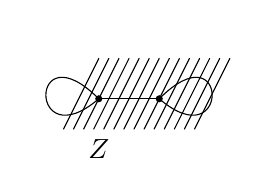
\begin{tikzpicture}[scale=.64,line cap=round,line join=round]\begin{scope}[shift={(0,0)}]\draw(0,0)--(1.2,0);\draw(0,0)..controls(-1.4,1.4)and(-1.4,-1.2)..(0,0);\draw(1.2,0)..controls(2.6,1.4)and(2.6,-1.2)..(1.2,0);\fill(0,0)circle(2pt);\fill(1.2,0)circle(2pt);\foreach\x in{-.7,-.5,...,2}\draw(\x,-.6)--(\x+.7,.8);\node at(0,-1){$\mathbb Z$};\end{scope}\end{tikzpicture}}}
\figure{\begin{tikzpicture}[scale=.64,line cap=round,line join=round]\begin{scope}[shift={(7,1)}]\draw(0,0)--(1.2,0);\draw(0,0)..controls(-1.4,1.4)and(-1.4,-1.2)..(0,0);\draw(1.2,0)..controls(2.6,1.4)and(2.6,-1.2)..(1.2,0);\fill(0,0)circle(2pt);\fill(1.2,0)circle(2pt);\node at(0,-1){$\mathbb Z_2\times\mathbb Z_2$};\end{scope}\begin{scope}[shift={(2,-1.4)}]\fill(0,0)circle(2pt);\draw(0,0)..controls(-1.3,1.4)and(-1.4,-1)..(0,0);\draw(0,0)--(1.2,0)--(1.8,.5);\draw(1.2,0)--(1.8,-.5);\fill(1.2,0)circle(2pt);\node at(0,-1){$\mathbb Z_2$};\end{scope}\begin{scope}[shift={(7,-1.4)}]\draw(-.7,.5)--(0,0)--(-.7,-.5);\draw(0,0)--(1,0);\draw(1.7,.5)--(1,0)--(1.7,-.5);\fill(0,0)circle(2pt);\fill(1,0)circle(2pt);\node at(0,-1){$\mathbb Z_2\times\mathbb Z_2$};\end{scope}\end{tikzpicture}}
\figure{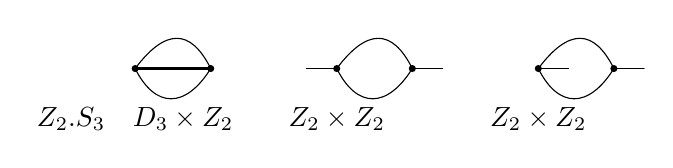
\begin{tikzpicture}[scale=.64,line cap=round,line join=round]\begin{scope}[shift={(0,0)}]\draw(0,0)..controls(.6,.8)and(1.1,.8)..(1.5,0)..controls(1,-.8)and(.4,-.8)..(0,0);\fill(0,0)circle(2pt);\fill(1.5,0)circle(2pt);\draw[thick](0,0)--(1.5,0);\node at(0,-1){$\mathbb Z_2.\mathfrak S_3\quad\deleted{\unsure{D_3\times\mathbb Z_2}}$};\end{scope}\begin{scope}[shift={(4,0)}]\draw(0,0)..controls(.6,.8)and(1.1,.8)..(1.5,0)..controls(1,-.8)and(.4,-.8)..(0,0);\fill(0,0)circle(2pt);\fill(1.5,0)circle(2pt);\draw(-.6,0)--(0,0);\draw(1.5,0)--(2.1,0);\node at(0,-1){$\mathbb Z_2\times\mathbb Z_2$};\end{scope}\begin{scope}[shift={(8,0)}]\draw(0,0)..controls(.6,.8)and(1.1,.8)..(1.5,0)..controls(1,-.8)and(.4,-.8)..(0,0);\fill(0,0)circle(2pt);\fill(1.5,0)circle(2pt);\draw(0,0)--(.6,0);\draw(1.5,0)--(2.1,0);\node at(0,-1){$\mathbb Z_2\times\mathbb Z_2$};\end{scope}\end{tikzpicture}}
